\documentclass{standalone}
\usepackage{tikz}
\usepackage{ctex,siunitx,ninecolors}
\setCJKmainfont{Noto Serif CJK SC}
\usepackage{tkz-euclide}
\usepackage{amsmath}
\usetikzlibrary{patterns, calc}
\usetikzlibrary {decorations.pathmorphing, decorations.pathreplacing, decorations.shapes}
\begin{document}
\small\linespread{1.0}
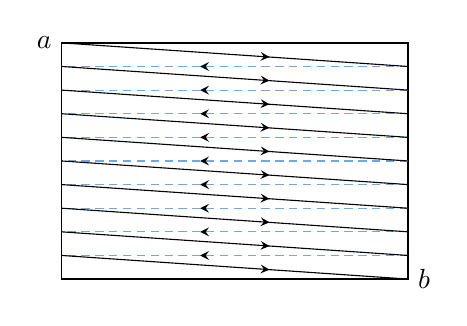
\begin{tikzpicture}[>=stealth]
  \draw[semithick](-2.2,1.5)node[left]{$a$}rectangle(2.2,-1.5)node[right]{$b$};
  \foreach \x in {-1.2,-0.9,...,1.3}
  {
    \draw[densely dashed,azure7,postaction={decorate},decoration={markings,mark={at position 0.6 with {\arrow[black]{>}}}}](2.2,\x)--(-2.2,\x);
    \draw[postaction={decorate},decoration={markings,mark={at position 0.6 with {\arrow[black]{>}}}}](-2.2,\x)--(2.2,\x-0.3);
  }
  \draw[postaction={decorate},decoration={markings,mark={at position 0.6 with {\arrow[black]{>}}}}](-2.2,1.5)--(2.2,1.2);
\end{tikzpicture}
\end{document}